\documentclass[a4paper]{article} %%% use \documentstyle for old LaTeX compilers

\usepackage[portuguese]{babel} %%% 'french', 'german', 'spanish', 'danish', etc.
\usepackage{makeidx}
\usepackage{multirow}
\usepackage{multicol}
\usepackage[dvipsnames,svgnames,table]{xcolor}
\usepackage[dvips]{graphicx} 
\usepackage[utf8x]{inputenc}
\usepackage{epstopdf}
\usepackage{ulem}
\usepackage{hyperref}
\usepackage{amsmath}
\usepackage{amssymb}
\usepackage{txfonts}
\usepackage{mathdots}
\usepackage[classicReIm]{kpfonts}

% You can include more LaTeX packages here 

\usepackage[a4paper,top=2.5cm,bottom=2.5cm,left=3cm,right=3cm,marginparwidth=1.75cm]{geometry}
\begin{document}

%\selectlanguage{english} %%% remove comment delimiter ('%') and select language if required

\title{Projeto final}
\author{Bruno da silva}

\fontfamily{phv}\selectfont
\begin{titlepage}
	\begin{center}
		{\scshape\Large Universidade Federal Fluminense -UFF \par}
		\vspace{7cm}
		{\huge\bfseries Soluções de problemas físicos com método de Verlet  \par}
		\vspace{5.5cm}
		{\itshape Autor Bruno da Silva Machado \par}      
		
		\vspace{6.5cm}    
		
		\vfill
		{\large \today\par}
	\end{center}
\end{titlepage}

\tableofcontents{}

\newpage

\section*{Abstract}
\noindent

in this article will be analyzed problems physical of origin dynamic as a oscillator coupled, double pendulum and oscillator mass spring that rotaciona in axis, from their equations of motion, in order to develop an algorithm computational with the finality of use a method of verlet and simulate the displacement of this with demonstration

keywords: problems physical; Numerical methods.

\section*{Resumo}

No presente artigo serão analisados problemas físicos de origem dinâmica como um oscilador acoplado, pêndulo duplo e oscilador massa mola que rotaciona no eixo, a partir de suas equações do movimento, afim de desenvolver um algoritmo computacional com finalidade de utilizar um método de Verlet e simular os deslocamentos destes com demonstração gráfica.

Palavras-chave: Problemas físicos; M\'{e}todos num\'{e}ricos.


\section*{Introdu\c{c}\~{a}o}

\noindent

Na F\'{i}sica e Matem\'{a}tica, na \'{a}rea de sistemas din\^{a}micos, um p\^{e}ndulo duplo \'{e} um sistema com dois p\^{e}ndulos sendo um deles anexo no extremo do outro. Este \'{e} um sistema f\'{i}sico simples que apresentam um complexo comportamento din\^{a}mico com alta sensibilidade em torno das condi\c{c}\~{o}es iniciais. O movimento do p\^{e}ndulo duplo \'{e} regido por um conjunto fechado de equa\c{c}\~{o}es diferenciais ordin\'{a}rias. Para sistemas com energia espec\'{i}fica, seu comportamento \'{e} ca\'{o}tico.

No caso do oscilador acoplado temos uma conjunto de pêndulos ou blocos de massas diferentes interligador por uma mola e separados por uma distancia d este pode oscilar ou não harmonicamente e podem possuir massa distintas entre si ou estarem em bases ou haste de tamanho diferente.

Usaremos o m\'{e}todo de Verlet por sua simplicidade e estabilidade por nos fornece uma boa aproxima\c{c}\~{a}o num\'{e}rica para o problema em questão.
\newpage

\noindent 
\section{Oscilações Acopladas}\label{sec:intro}

\noindent 

Consideremos um sistema de dois pêndulos ligados por uma mola e sujeitos a oscilar no plano vertical definido pelas suas posições de equilíbrio. A distância d entre os pêndulos, na posição de equilíbrio, é igual ao comprimento natural da mola, de modo que, nessa posição, ela não se encontra comprimida nem esticada; seja k a constante elástica da mola. Se a massa M suspensa de um m dos pêndulos é muito maior que a massa m do outro, temos um típico problema de oscilações forçadas: as oscilações do pêndulo pesado, transmitidas através da mola, atuam sobre o pêndulo leve como uma força externa, forçando-o a oscilar com a frequência do pêndulo pesado. 
O problema se toma mais interessante quando os pêndulos acoplados são idênticos, ou seja, têm mesmo comprimento b e mesma massa m. Terão portanto também a mesma frequência angular de oscilação livre, que, para pequenas oscilações, é dada por $\omega_0^2 = g/l$


\begin{center}
	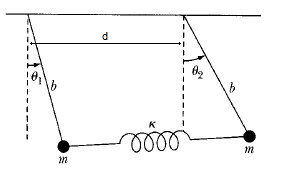
\includegraphics[width=2.82in, height=1.73in, keepaspectratio=false]{Oscilador.PNG}
	
	\scriptsize{ Figura1. Oscilador acoplado. nesta figura temos dois pêndulos de comprimentos iguais possuindo massa iguais são conectados por uma mola. }
\end{center}

\subsection{Solução do oscilador acoplado}

Oscilador acoplado pode ser solucionado através da abordagem das leis de Newton mas para uma solução geral essa estrategia não e muito útil uma vez que as equações se tornam cada vez mais complexa. Enfim de apresentar uma solução mais geral para o oscilador acoplado usaremos a mecânica Lagrangiana.

Considere dois pêndulos de massa e comprimentos iguais ligador por uma mola como na figura acima através da mecânica lagrangiana podemos soluciona -los obtendo as suas energias cinéticas e potenciais
Assim a energia cinética do sistema e a soma das energias individuais de cada pendulo.
\[T = \frac{1}{2}mb\dot{\theta_1}^2 + \frac{1}{2}mb\dot{\theta_2}^2\] 

e a energia potencial também sera combinação das energias.

\[U = mgb(1-\cos(\theta_1)) + mgb(1 -\cos(\theta_2))+\frac{1}{2}k(b\sin(\theta_1)+bsin(\theta_2))\]   
para pequenas oscilações temos $\sin(\theta) \approx \theta$ e $\cos(\theta) \approx 1 - \frac{\theta^2}{2}$ assim:
\[U = \frac{mgb(\theta_1^2+\theta_2^2)}{2} +\frac{1}{2}kb^2(\theta_1-\theta_2)\]

montando a lagrangiana temos
\[L = T - U\]
\[L = \frac{1}{2}mb\dot{\theta_1}^2 + \frac{1}{2}mb\dot{\theta_2}^2 - \frac{mgb(\theta_1^2+\theta_2^2)}{2} -\frac{1}{2}kb^2(\theta_1-\theta_2)\]

para $\theta_1$

\[\frac{\partial L}{\partial \theta_1} - \frac{d}{dt}\left(\frac{\partial L}{\partial \dot{\theta_1}}\right) = 0\]
\[-mgb\theta_1 -kb^2(\theta_1-\theta_2) -\frac{d}{dt}(mb^2\dot{\theta_1}) = 0\]
\[-mgb\theta_1 -kb^2(\theta_1-\theta_2) -mb^2\ddot{\theta_1} = 0\]
\[mb^2\ddot{\theta_1} +mgb\theta_1 +kb^2(\theta_1-\theta_2) = 0\]
\begin{equation}
	\ddot{\theta_1} + \frac{g}{b}\theta_1 + \frac{k}{m}(\theta_1-\theta_2) = 0
\end{equation}

para $\theta_2$

\[\frac{\partial L}{\partial \theta_2} - \frac{d}{dt}\left(\frac{\partial L}{\partial \dot{\theta_2}}\right) = 0\]
\[-mgb\theta_2 -kb^2(\theta_1-\theta_2) -\frac{d}{dt}(mb^2\dot{\theta_2}) = 0\]
\[-mgb\theta_2 -kb^2(\theta_1-\theta_2) -mb^2\ddot{\theta_2} = 0\]
\[mb^2\ddot{\theta_2} +mgb\theta_2 +kb^2(\theta_1-\theta_2) = 0\]
\begin{equation}
\ddot{\theta_2} + \frac{g}{b}\theta_2 + \frac{k}{m}(\theta_1-\theta_2) = 0
\end{equation}

observe que as nossa duas equações são acopladas ou seja o movimento de um depende do movimento do outro nesse caso como são apenas dois pêndulos fica fácil separar as duas equações

Somando membro a membro de (1) e (2) obtemos

\begin{equation}
(\ddot{\theta_1} + \ddot{\theta_2}) - \omega_0 ^2(\theta_1+\theta_2) -\frac{2k}{m}(\theta_1-\theta_2)
\end{equation} 

e agora subtraindo (1) de (2)
\begin{equation}
(\ddot{\theta_1} - \ddot{\theta_2}) + \omega_0 ^2(\theta_2-\theta_2) 
\end{equation}

assim obtemos:

\begin{equation}
\left\{\begin{array}{ll}q_1 = \frac{1}{2}(\theta_1+\theta_2) \\
q_2 = \frac{1}{2}(\theta_2-\theta_1)\end{array}\right
\end{equation}


\section{Oscilador massa mola}

Agora vamos considerar um oscilador massa mola que consiste em um bloco de peso qualquer ligado em uma mola de coeficiente k de massa desprezível oscilando em um plano sem atrito, mas agora temos um fator extra que e o fato do oscilador esta rodando ao redor do eixo de equilíbrio.
Outro fator que aumenta a complexidade e a mola do oscilado como ele esta em movimento, este em varias direções, tem o fato que a mola estica e se contra enquanto o bloco se movimenta no plano o que faz com que o movimento dependa não só do sentido da rotação mas também o estado da mola sendo este o principal modificador da direção do bloco  

\begin{center}
	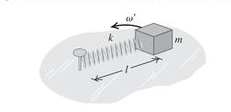
\includegraphics[width=2.31in, height=1.12in, keepaspectratio=false]{oscilador_r.png}
	
	\scriptsize{ Figura2. Oscilador ligado em uma mola que efetua uma rotação ao redor do eixo de equilíbrio}
\end{center} 

\subsection{Solução do oscilador}
A partir das informações acima obtemos o seguinte sistema

\begin{equation}
\left\{\begin{array}{ll} x = l\cos(\theta) \\
 y = l\sin(\theta)\end{array}\right
\end{equation}

\begin{equation}
\left\{\begin{array}{ll} \dot{x} = \dot{l}\cos(\theta) -l\dot{\theta}\sin(\theta)\\
\dot{y} = \dot{l}\sin(\theta) -l\dot{\theta}\cos(\theta)\end{array}\right
\end{equation}

utilizando os métodos da mecânica lagrangiana temos para:

energia cinética:
\[T = \frac{1}{2}m\dot{x}^2+\frac{1}{2}m\dot{y}^2\]
\[\frac{1}{2}m(\dot{l}\cos(\theta) -l\dot{\theta}\sin(\theta))^2 + \frac{1}{2}m(\dot{l}\sin(\theta) -l\dot{\theta}\cos(\theta))^2\]
\[T = \frac{1}{2}m(\dot{l}^2 + l^2\dot{\theta}^2)\]

energia potencial:
\[U = mgl\sin(\theta) +  \frac{1}{2}k(l-b)^2\]

assim tomamos a lagrangiana
\[\mathcal{L} = \frac{1}{2}m(\dot{l}^2 + l^2\dot{\theta)}^2 - mgl\sin(\theta) - \frac{1}{2}k(l-b)^2\]

solucionado para l:
\[\frac{\partial \mathcal{L}}{\partial \l} - \frac{d}{dt}\left(\frac{\partial \mathcal{L}}{\partial \dot{\l}}\right) = 0\]

\[mb\dot{\theta}^2 -mg\cos(\theta) -k(l-b) -\frac{d}{dt}(m\dot{l}) = 0\]
\[mb\dot{\theta}^2 -mg\cos(\theta) -k(l-b) -m\ddot{l} = 0\]

\begin{equation}
	\ddot{l} = l\dot{\theta}^2 -g\cos(\theta) -\frac{k}{m}(l-b)
\end{equation}


para $\theta$
\[\frac{\partial \mathcal{L}}{\partial \theta} - \frac{d}{dt}\left(\frac{\partial \mathcal{L}}{\partial \dot{\theta}}\right) = 0\]
\[mgl\cos(\theta) -\frac{d}{dt}(ml^2\dot{\theta}) = 0\]
\[mgl\cos(\theta) -2ml\dot{l}\dot{\theta} - ml^2\ddot{\theta} = 0\]
\begin{equation}
	\ddot{\theta} =  \frac{g}{l}\cos(\theta) - \frac{2}{l}\dot{l}\dot{\theta}
\end{equation}

Note que novamente chegamos em duas equações diferenciais só que dessa vez restringimos a posição no plano e uma depende da outra.

\section{Pendulo duplo}

O modelo utilizado, consiste em p\^{e}ndulo duplo, que nada mais \'{e} do que um p\^{e}ndulo simples acoplado a outro, na Figura 1 \'{e} representa\c{c}\~{a}o do modelo implementado.

\begin{center}
	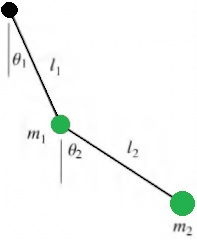
\includegraphics[width=3.00in, height=2.50in, keepaspectratio=false]{Fimage5.jpg}
	
	\scriptsize {Figura3. Modelo do p\^{e}ndulo duplo.}
\end{center}


Esse p\'{e}ndulo duplo \'{e} composto por duas massas $\ m_1 $ e $\ m_2$ conectadas por hastes de massas desprez\'{i}veis de comprimento $\ l_1$ e $\ l_2$, os \^{a}ngulos utilizados s\~{a}o $\theta_1$ e $\theta_2$, e a acelera\c{c}\~{a}o da gravidade \'{e} $\ g = 9,81 m/s^2$
Podemos dizer que o corpo de massa $\ m_1$ gira em torno de um ponto fixo (representado pelo circulo preto), sendo este um referencial inercial, diferentemente da massa $\ m_2$ que gira em torno da massa $\ m_1$ utilizando um sistema de referencia relativa.

\subsection{Equa\c{c}\~{o}es do movimento}

Para deduzir as equa\c{c}\~{o}es do p\^{e}dulo duplo usaremos uma ferramenta da mec\^{a}nica cl\'{a}ssica para abordar sistemas complexos que \'{e} o lagrangiano  pode ser descrito como a diferen\c{c}a entre energia cinetica pela energia potencial do sistema.

A partir do lagrangiano podemos deduzir as equa\c{c}\~{o}es de movimento do sistema.
seja $\dot{\theta_1}$ e $\ddot{\theta_1}$ derivada temporal em relação a $\theta_1$ temos para $\theta_1$:
\[\frac{\partial{\mathcal{L}}}{\partial \dot{\theta_1}} = (m_1+m_2)l_1^{2}\dot{\theta_1}+m_2l_1l_2\dot{\theta_2}\cos(\theta_1-\theta_2)\]
\[\frac{d}{dt}\left(\frac{\partial{\mathcal{L}}}{\partial{\dot{\theta_1}}}\right) = (m_1+m_2)l_1^{2}\ddot{\theta_1}+m_2l_1l_2\ddot{\theta_2}\cos(\theta_1-\theta_2) - m_2l_1l_2\dot{\theta_2}\sin(\theta_1-\theta_2)(\dot{\theta_1} - \dot{\theta_2})\]
\begin{equation}
	\frac{\partial{\mathcal{L}}}{\partial \dot{\theta_1}} = -l_1g(m_1+m_2)\sin(\theta_1) -m_2l_1l_2\dot{\theta_1}\dot{\theta_2}\sin(\theta_1-\theta_2)
\end{equation}
toma assim a forma:

\[(m_1+m_2)l_1^2\ddot{\theta_1} + m_2l_1l_2\ddot{\theta_2}cos(\theta_1 - \theta_2)+m_2l_1l_2\dot{\theta_2^{2}}\sin(\theta_1-\theta_2)+l_1g(m1+m2)\sin(\theta_1) = 0 \]

simplificamos temos:
\[(m_1+m_2)l_1\ddot{\theta_1} + m_2l_2\ddot{\theta_2}cos(\theta_1 - \theta_2)+m_2l_2\dot{\theta_2^{2}}\sin(\theta_1-\theta_2)+g(m1+m2)\sin(\theta_1) = 0 \]

E para $\theta_2$:
\[\frac{\partial{\mathcal{L}}}{\partial \dot{\theta_2}} = m_2l_2^{2}\dot{\theta_2}+m_2l_1l_2\dot{\theta_1}\cos(\theta_1-\theta_2)\]
\[\frac{d}{dt}\left(\frac{\partial{\mathcal{L}}}{\partial{\dot{\theta_2}}}\right) = (m_1+m_2)l_2^{2}\ddot{\theta_2}+m_2l_1l_2\ddot{\theta_1}\cos(\theta_1-\theta_2) - m_2l_1l_2\dot{\theta_1}\sin(\theta_1-\theta_2)(\dot{\theta_1} - \dot{\theta_2})\]
\[\frac{\partial{\mathcal{L}}}{\partial \dot{\theta_2}} = m_2l_1l_2\dot{\theta_1}\dot{\theta_2}\sin(\theta_1-\theta_2) -l_2gm_2\sin(\theta_2)\]

simplificando por $\ l_2$
\begin{equation}
	m_2l_2\ddot{\theta_2}+m_2l_1\dot{\theta_1}\cos(\theta_1-\theta_2) -m_2l_1\dot{\theta_1^{2}}\sin(\theta_1-\theta_2)+m_2g\sin(\theta_2) = 0  
\end{equation}
 

Os sistemas de equa\c{c}\~{o}es diferenciais de segunda ordem formado por (10) e (11) pode ser resolvido numericamente em ordem de $\theta_1(t)$ e $\theta_2(t)$

\section{Resultados}

A partir das relações anteriores podemos chegar nas solu\c{c}\~{o}es num\'{e}ricas usando o método de verlet. Para avaliar o que obtemos vamos exemplifica-lo.

\subsection{Resultados do oscilador acoplado}

Seja os pêndulos p1 e p2 com massa de 0.25kg possuindo uma haste de 0.5m partindo do repouso com ângulos iguais de $\pi/2$ sendo a velocidade inicial de p1 = 0 m/s e p2 = 0.1 m/s, obtemos os seguintes gráficos 
\vspace{0.5cm}
\begin{center}
	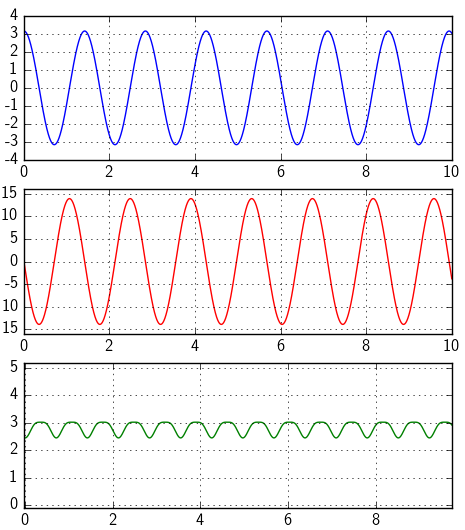
\includegraphics[width=4.65in,height=5.30in, keepaspectratio=true]{pendulo_acoplado.PNG}
	
	\scriptsize{Figura 4. gráficos da posição da velocidade e da energia em relação ao tempo}
\end{center}

Como podemos ver acima o gráfico da posição,(azul), se parece com uma senoide de modo que varie uniformemente com o tempo apesar de não visível este gráfico e uma sobreposição das posições de p1 e p2 em relação do tempo e como ele possui este formato característico podemos concluir que o movimento e harmônico.

No caso do gráfico da velocidade,(vermelho), podemos notar que este gráfico também é uma senoide mas, diferente do outro este inicia o movimento aproximadamente do zero e não é só isso por ser um gráfico da sobreposição da velocidade de p1 e p2 podemos supor que para ter este formato as velocidades de p1 e p2 deveriam oscilar harmonicamente de modo que quando p2 é máximo p1 é minimo e vice versa

E o nosso ultimo gráfico é a da energia,(verde), e notável que o gráfico da energia esteja 'pulsando' com o tempo, ou seja, a um ganho de energia até um valor limite depois disso se mantem constante e rapidamente a uma 'perda' de energia até um valor minimo e este padrão se repete periodicamente como este gráfico também é uma sopre posição podemos partir da hipótese que os ganhos e perdas na verdade são transferências de energia de um pendulo para o outro sendo que esta não se dá de imediato uma vez que há uma transformação de energia cinética para potencial elástica e vice versa de modo que nos momentos constantes no gráfico um dos pêndulos possui toda a energia do sistema e o outro esta em repouso mas este efeito é rapidamente 'quebrado' de modo que haja um fluxo constante da energia total do sistema e se isso for verdade obtemos assim a conservação de energia no  sistema garantindo a validade dos resultado  anteriores. 

Agora partimos de uma situação um pouco diferente usando p1 e p2 do exemplo anterior só que desta vez p2 parti de um angulo de $-\pi/2$ e p1 partindo do sentido oposto.
\vspace{1cm}

\begin{center}
	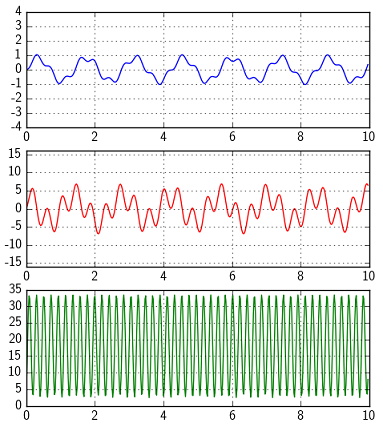
\includegraphics[width=3.38in,height=4.27in, keepaspectratio=false]{pendulo_acoplado2.PNG}
	
	\scriptsize {Figura 5.para uma mudança de direção tivemos uma mudança brusca nos resultado.}
\end{center}

Como podemos ver uma simples mudança de ângulos iniciais fez com que o comportamento ficasse completamente diferente do anterior. Para o gráfico da posição,(em azul), vemos que o seu comportamento difere muito do gráfico anterior de modo que não podemos descrever a sua curva sem antes uma analise previa. Como já sabemos esta curva é uma sobreposição das posições de p1 e p2 sendo assim podemos supor que a mudança nas posições inicias afetam o sistema e como eles partiram de sentidos opostos houve uma interferência não construtiva entre os pêndulos e o fato de não se anularem e bem simples um deles partiu com velocidade maior que o outro e ambos estão devassados por uma fase de $\pi/2$. Agora dando uma olhada criteriosa vemos que o movimento não e mais harmônico simples porém é periódico isto e notado pelo fato da curva se repetir ao longo do tempo.

Agora vamos analisar o gráfico da velocidade v,(verde), vemos que ele tem um comportamento similar ao da posição mas, para descrever -lo vamos analisar o que ocorre nos pontos de máximos e mínimos locais da curva. Vemos que não é todo pico no gráfico que é uma máximo ou minimo porem esta informação não nos ajuda muito sendo assim vamos olhar os pontos que realmente são picos na curva neles esperamos obviamente que sejam a velocidade máxima e minima do sistema e que o corram isso ocorram nos extremos das trajetórias dos pêndulos uma vez que estão acoplados e supomos de maneira análoga que quando $v = min$ e $v = max$ eles estejam extremamente afastados ou próximos respectivamente.

E por fim vamos analisar o gráfico da energia total do sistema bem diferente do anterior este parece oscilar constantemente de maneira quando estão extremamente afastados ou próximos a energia é minima ou máxima respectivamente de modo que este eventos extremo ocorram de maneira rápida as outras regiões da curva são de transição entre estes extremos.

Para finalizar esta analise do oscilador acoplado vamos ver o espaço de fase de sobreposição entre eles.

O primeiro e para o caso em que p1 e p2 partem com angulo de $\pi/2$ em relação ao ponto de equilíbrio  

\begin{center}
	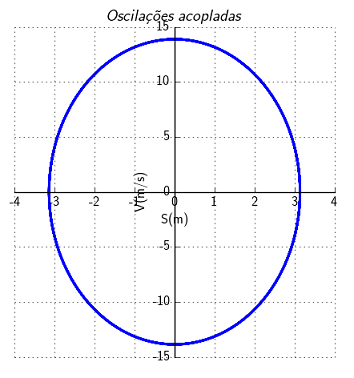
\includegraphics[width=3.54in,height=3.78in, keepaspectratio=false]{pendulo_acoplado4.PNG}
	
	\scriptsize {Figura 6. Espaço de fase da sobreposição dos pêndulos }
\end{center}

É notável e interessante que o espaço de fase seja uma elipse isso nos mostra que o movimento não se da de forma uniforme porem, este tem que percorre áreas iguais no mesmo intervalo de tempo se que este movimento seja harmônico isto nos revela que os pontos extremos no eixo V do gráfico a velocidade deve ser minimo e os ponto que cortam o eixo S a velocidade deve ser máxima de modo que as regiões entre estes extremos sejam de transição, são nelas em que os pêndulos estão em movimento visto que nos extremos eles alcançam o limite da trajetória. E como a curva e fechada podemos confirmar que a energia se conserva e não só isso por ser uma quádrica isto revela também que o movimento é harmônico validando os resultados obtido e mostrados na figura 4. 

O segundo caso  e para  p1 partindo com angulo de $-\pi/2$ e p2 $\pi/2$ em relação a posição de equilíbrio.

\begin{center}
	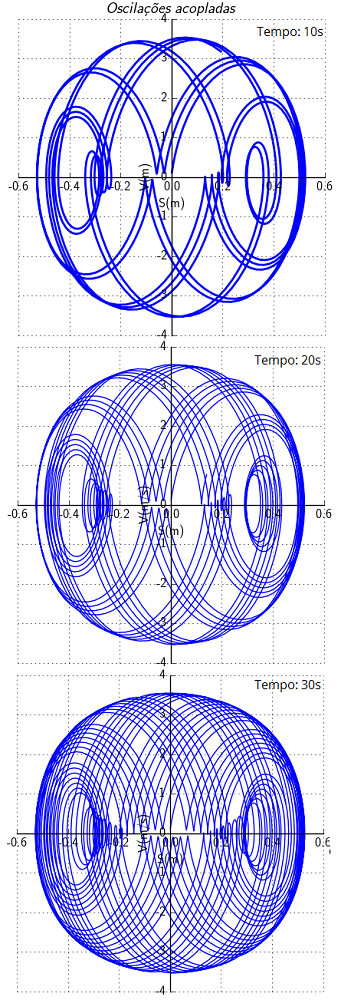
\includegraphics[width=3.41in,height=10.00in, keepaspectratio=false]{pendulo_acoplado7.PNG}
	
	\scriptsize{Figura 7. Espaço de fase da sobreposição dos pêndulos com angulo inicial opostos e iguais em modulo.}
\end{center}

Não tão surpreendente o espaço de fase do segundo caso é completamente diferente do primeira e também mais complexo podemos ver que o seu movimento não é harmônico pois percorre diversos cominhos distintos ao de correr do tempo e também vemos que este não pode ser descrito por uma quádrica mas por uma sobreposição destas também e possível notar que ela é alongada no eixo V e um pouco achatado no eixo S de modo que ela apresenta características similares ao gráfico anterior assim podemos supor que ela apresente os mesmo comportamentos nos extremos. Apesar de não ser um movimento harmônico ele é periódico como nós suspeitávamos ao olhar para os gráficos de posição e velocidade  podemos ver que o formato da curva se repete nas mesmas regiões no gráfico e apesar de ser discreto é possível notar que este gráfico possui um raio de limitador ou seja a curva nunca ultrapassa determinada região e este raio limitador é uma elipse centrada na origem  $ \left(\frac{x}{3.5}\right)^2 +  \left(\frac{y}{5}\right)^2 = 1 $ como ele possui um valor limite no espaço de fase de modo que a curva não seja aberta temos que a energia se conserva.  

\subsection{Resultados do oscilador massa mola}
\noindent

Seja um bloco de massa 1 kg preso a extremidade de uma mola sem massa cuja a constante é 25 e comprimento de equilíbrio é 3 cm e pode girar livremente em torno de um prego cravado em uma superfície sem atrito. A partir dessa informações obtemos os seguintes gráficos 
\vspace{1cm} 
\begin{center}
	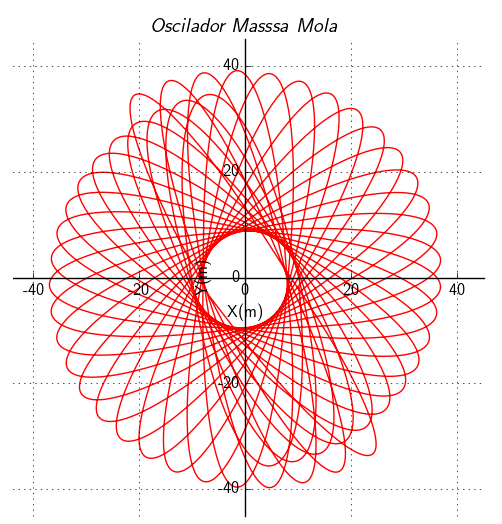
\includegraphics[width=5.02in,height=5.24in, keepaspectratio=false]{penMassaMola.png}
	
	\scriptsize {Figura 8. gráfico da posição do oscilador}
\end{center}

como podemos ver o gráfico da posição possui um formato de tório isso decore do fato do bloco não só esta oscilando mas também esta girando ao redor do eixo de equilíbrio. podemos ver também,apesar de discreto, que a amplitude não se mantem com o tempo uma vez que a mola vai esticando com ou aumento da velocidade.

o próximo gráfico é o da velocidade.
\vspace{1cm}
\begin{center}
	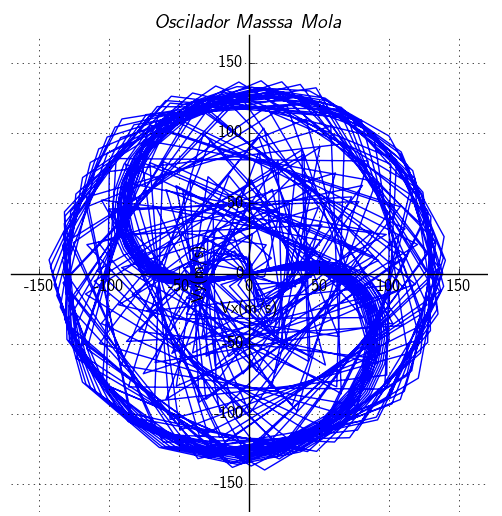
\includegraphics[width=5.02in,height=5.16in, keepaspectratio=false]{penMassaMolaVxy.png}
	
	\scriptsize {Figura 9. Gráfico da velocidade.}
\end{center}

Ele é notavelmente caótico, há 'quebras' no sentido da velocidade em praticamente todos máximos e mínimos locais apesar disso ele vai tentando descrever um vórtex na direção da origem  estas quebras o correm devido a mudança constante e  força da da direção causada pela mola e a rotação ao redor do eixo. Ele também possui um raio limite ele esta contido em uma circunferencial de raio 150.

E por fim vamos analisar o seu espaço de fase.

\begin{center}
	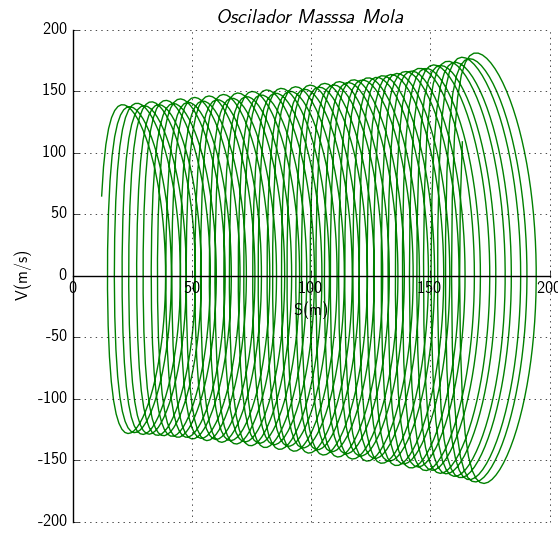
\includegraphics[width=5.58in,height=5.36in, keepaspectratio=false]{penMassaMolaXV.png}
	
	\scriptsize {Figura 10. Gráfico do espaço de fase.}
\end{center}

E realmente interessante este espaço de fase pois ele tem um formato de uma espira e esta vai se alongando e aumentando o raio par toda a região positiva do gráfico e incrivelmente surpreendente que relação em a velocidade que é um gráfico caótico e cheio de descontinuidades, e a posição que é uma curva fechada resulte em uma curva suave e aberta, contudo por ser não sr fechada isso nos revela que a energia não se conserva e que este movimento não é harmônico e nem periódico.    

\subsection{Resultados do pendulo duplo}

Como j\'{a} foi dito na se\c{c}\~{a}o anterior(3.1), p\^{e}ndulo duplo leva-nos a equa\c{c}\~{o}es que s\'{o} podem ser resolvidas numericamente

\subsubsection{Solu\c{c}\~{a}o por m\'{e}todos n\'{u}mericos}
Agora vamos dividir o nosso problema em dois sistemas diferentes. O primeiro relaciona $\theta_1$
e $\theta_2$ com as suas derivadas $\dot{\theta_1}$ e $\dot{\theta_2}$ A solu\c{c}\~{a}o num\'{e}rica \'{e} trivialmente simples:
\[\theta_{1,j} = \theta_{1,j-1} + \dot{\theta}_{1,j}\Delta{t} + \frac{1}{2}\ddot{\theta}_{1,j}\Delta{t}^2 \]
\[\theta_{2,j} = \theta_{2,j-1} + \dot{\theta}_{2,j}\Delta{t} + \frac{1}{2}\ddot{\theta}_{2,j}\Delta{t}^2 \]

E o resto n\~{a}o \'{e} t\~{a}o f\'{a}cil. Comecemos por estabelecer $\omega \equiv \dot{\theta} $ e, consequentemente, $\dot{\omega} = \ddot{\theta}$. Resolvendo o sistema de equa\c{c}\~{o}es formado por (12) e (13) em ordem a $\theta_1$ e $\theta_2$
obtemos:

\[\dot{\omega_1} = \frac{-g(2m_1+m_2)\sin(\theta_1)-m_2g\sin(\theta_1 - 2\theta_2)-2\sin(\theta_1-\theta_2)m_2(\omega_2^2l_2-\omega_1^2l_1\cos(\theta_1-\theta_2))}{l1(2m_1 + m_2 -m_2\cos(2\theta_1-2\theta_2))}\]
\[\dot{\omega_2} = \frac{2\sin(\theta_1-\theta_2)(\omega_1^{2}l_1(m_1+m_2)+g(m_1+m_2)\cos(\omega_1)+\omega_2^{2}l_2m_2\cos(\theta_1-\theta_2) }{l_2(2m_1+m_2-m_2\cos(2\theta_1-2\theta_2))}\]

Agora vamos exemplificar o nossa solução através da seguintes condições iniciais:

- os \^{a}ngulos $\theta_1$ = -0,785 rad, $\theta_2$ = 0,785 rad
- velocidades angulares iniciais igual a zero $\dot{\theta_1} = 0 rad/s, \dot{\theta_2} = 0 rad/s$
- Massas, $\ m_1 = 1.0kg e m_2 = 1.0kg$
-Acelera\c{c}\~{a}o da gravidade, $\ g = 9,81 m/s^2$
-Haste $l_1 = l_2 =$ 0,5m 
 \vspace{1cm} 
\begin{center}
	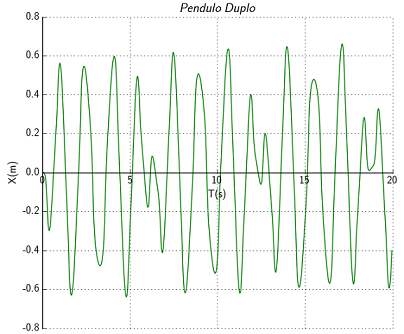
\includegraphics[width=4.04in,height=3.34in, keepaspectratio=false]{pendulo_duploTX.png}
	
	\scriptsize {Figura 11.comportamento do angulo$\theta_2$ em fun\c{c}\~{a}o do tempo.}
\end{center}

\begin{center}
	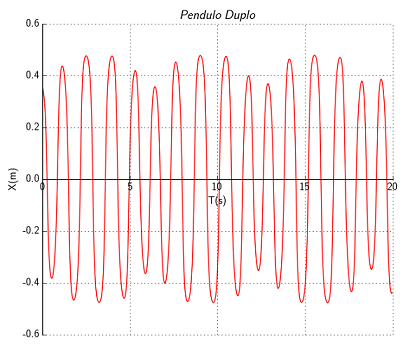
\includegraphics[width=4.03in,height=3.46in, keepaspectratio=false]{pendulo_duploTX2.png}
	
	\scriptsize {Figura 12.comportamento do angulo$\theta_1$ em fun\c{c}\~{a}o do tempo}
\end{center}

No primeiro gráfico temos um comportamento caótico do pendulo m2 isto ocorre por ser sensível as condições iniciais de maneira que o seu comportamento muda ao longo do tempo diferente do segundo gráfico em que oscila de maneira periódica apesar da amplitude não ser constante o que nos revela que o movimento em m1 não e harmônico. 

Agora veremos as trajetórias que m1 e m2 descreve no plano XY: 
  

\begin{center}
	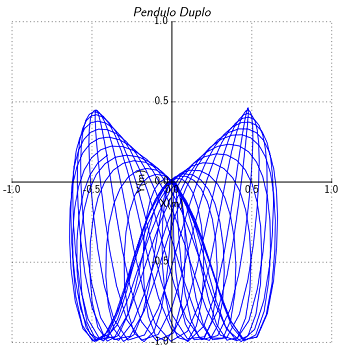
\includegraphics[width=3.51in,height=3.53in, keepaspectratio=false]{pendulo_duploXY.png}
	
	\scriptsize {Figura 13. a trajetória de m1 vemos que ela e caótica}
\end{center}

\begin{center}
		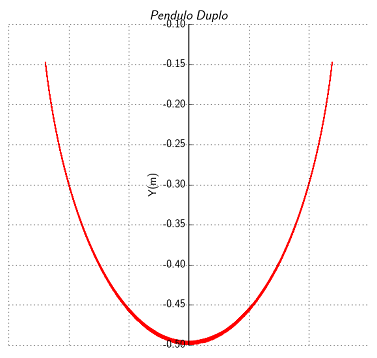
\includegraphics[width=3.77in,height=3.58in, keepaspectratio=false]{pendulo_duploXY2.png}
	
	\scriptsize {Figura 14. Trajetória de m2 vemos que ela e bem simples e comportada.}
\end{center}
Podemos ver e confirmar o que foi dito anteriormente uma vez que a sua trajetória e totalmente imprevisível em um longo período de tempo vemos que ele descreve varias curvas e  A cada ciclo a massa percorre um caminho distinto e apenas uma \'{u}nica vez.  Diferentemente o segundo gráfico é um arco de parábola sendo que este oscila com maior frequência no seu vértice que é o ponto de equilíbrio estável.

\section{Conclus\~{a}o}

Interpretação física 
Vemos que as soluções (1) e (2)  não correspondem em geral a MHS para $\theta_1$ e $\theta_2$: os deslocamentos são superposições de oscilações com frequências diferentes. Entretanto, existem duas novas coordenadas q1 e q2 , combinações lineares de $\theta_1$ e $\theta_2$, as quais oscilam harmonicamente. Essas denominam-se coordenadas normais. No presente caso, elas têm uma interpretação física simples: as (5) mostram que q1 é o \textit{deslocamento do centro de massa}, e 2q2 = $\theta_1$ - $\theta_2$ é o \textit{deslocamento relativo entre as duas partículas}, correspondendo à deformação da mola. Nas coordenadas normais, o sistema se desacopla. 

Neste estudo consideramos as massas $m_1$ e $m_2$ do pendulo como part\'{i}culas para nossa deduções o que facilitou bastante utilizamos o m\'{e}todo de Verlet mas poderíamos ter usado um mais sofisticado como Ruge-Kutta. Os resultados da implementação computacional foram obtidos resolvendo-se as equações de movimento com resultados gr\'{a}ficos que podem ser comparados de outros livros como Santos(2001)
Através desse estudo é evidenciado que o pêndulo duplo depende certamente das condições iniciais do sistema, pois se alterada essas temos mudança no movimento.
Portanto pode-se dizer que muitas vezes um programa computacional é mais viável, pois pode-se analisar um projeto antes de ser efetivado. Os resultados obtidos são muito próximos do real o que faz com que o programa está dentro condições reais.

\section*{Refer\^{e}ncias}

\noindent 

\indent N. J. Giordano \& H. Nakanishi, Computational Physics, 2${}^\circ$ed, 2007

\indent M\'etodo de Verlet, Wikip\'edia a enciclop\'edia livre, 2017

\indent Nussenzveig, Moyses, Curso de Física Básica 2, 3° ed, 1996

\indent Sears \& Zemansky, F\'{i}sica 2 Termodin\^{a}mica e ondas, 12${}^\circ$ed, 2008

\indent E.W. Weisstein, Double Pendulum, Eric Weisstein’s World of Physics, Wolfram Research.
 
\indent E. Neumann, Double Pendulum Physics Simulation, My Physics Lab,(2004).
 
\indent SANTOS, I.F., Din\^{a}mica de sistemas mec\^{a}nicos- modelagem simula\c{c}\~{a}o visualização verifica\c{c}\~{a}o.(S\~{a}o Paulo , 2001) p.65-84


\end{document}

